\documentclass[11pt,twocolumn]{article}
\bibliographystyle{siam}

\usepackage[margin=0.75in]{geometry}
\usepackage{graphicx}

\title{\textbf{Team Zeta Project Report}\\
Linear Modeling and Time Series Analysis of Visual Pattern Recognition}\\
\author{
  Chen, Tzu-Chieh\\
  \texttt{tcchenbtx}
  \and
  Ho, Edith\\
  \texttt{edithhcw}
  \and
  Marediya, Zubair\\
  \texttt{zubair-marediya}
  \and
  Tran, Mike\\
  \texttt{miketranx4}
  \and
  Zhang, Dongping\\
  \texttt{dpzhang}
}

\begin{document}
\maketitle

\abstract{}
If we present different types of 
visual stimulus to a subject, would each stimulus evoke the 
same category-specific pattern of response in the ventral object vision 
pathway? Furthermore, can we determine and predict individual
categories from the patterns of response evoked? 

\section{Introduction}

In Haxby et al's study, \emph{Distributed and Overlapping Representations of Faces
and Objects in Ventral Temporal Cortex}\cite{objectrec}, researchers collected data 
from six subjects, including five females and one male. 
Different categories of pictures were presented to subjects as visual stimuli.
The categories are faces, cats, chairs, shoes, bottles, tools, houses, 
and a control category of phase-scrambled images.
The study aimed to answer the following questions: if we present 
different categories of visual stimuli to a subject, will category-specific response be 
evoked in the ventral cortex? \\

Each subject was placed into a functional magnetic resonance imaging 
(fMRI) facility for 12 times. One complete experiment run lasted 300s. It began 
with 12s of rest, followed by 8 stimulus blocks of 24s duration, one for 
each category of visual stimuli. There were 12s intervals of rest between 
every two blocks, and the whole procedure ended with another 12s of rest. 
Each picture stimulus were presented for 0.5s followed by an inter-stimulus 
interval of 1.5ms. 12 stimuli were presented during each stimulus 
block, and a total of 96 stimuli in a complete experiment run.\\

In the study, the data collected for each subject were split into two 
runs: odd runs and even runs. Correlation was used as the indication of 
response similarity. Results from analyzing within-category and 
between-category correlations suggest that a lot of response patterns 
are overlapping. In the overlaps, there are parts of the cortex that respond 
more to a certain stimuli than others. The study defines these responses as 
maximal response. In order to gain more insights from the non-overlapping 
parts of the responses, the study tests whether the patterns of non-maximal 
responses carry category-related information. Voxels that responded maximally 
to were excluded from this calculation of correlations. The results show that the 
removal of maximally responsive voxels from correlation calculations 
barely diminishes the accuracy of identification. The study concludes 
that both the pattern of large and small responses and the location 
of large responses carry category-related information; and small responses 
are an integral part of the representation.\\

\section{Data}

The study's curated dataset can be found and downloaded on the OpenfMRI 
database with ds105's accession number. The ds105 
sub-directory contains files detailing this study, including general information 
(README file), related research articles (references.txt), detail information 
and update for this released dataset (release\textunderscore history.txt), 
the MR repetition time (scan\textunderscore key.txt), the name 
(study\textunderscore key.txt), and the major task for this study 
(object viewing) (task\textunderscore key.txt). In addition, the models folder 
contains files with the key conditions (list of object categories) 
(condition\textunderscore key.txt) and the comparison setting in this study 
(tast\textunderscore contrasts.txt). \\

Subjects have individual directories storing their results. There are four 
sub-directories in each of the respective directories. The anatomy 
sub-directory contains high-resolution scans of the subject's head 
(highres001.nii.gz), mask for obtaining the ``brain only'' scans 
(highres001\textunderscore brain\textunderscore mask.nii.gz), and the 
``brain only'' anatomy result (highres001\textunderscore brain.nii.gz). 
The ``behav" sub-directory is empty since subject's behavior is irrelevant 
to this study. The ``model" sub-directory provides information such as the 
onset time (in seconds), and the duration and weighting for each conditions 
(object category) for the 12 task runs in this study. The ``BOLD" sub-directory 
contains fMRI results for all 12 task runs for each subject respectively. 
In each task run directory, we can find the fMRI result (bold.nii.gz) and 
a QA sub-directory with that run's time series analysis report, fMRI results
pre-processing and confound files, and visualization of the brain (nii files).\\ 

\section{Methods}

For each subject, there are eight condition files corresponding 
to each of the eight objects for each of the twelve runs. Each
condition file consists of time points of when the object was presented 
during the run. We started our analysis with subject 1, where we first wrote 
helper functions to identify and remove outliers.  Then we ran 
the event2neural function on subject 1's condition files, which returned an 
array of 121 zeros or ones. These values indicate
time intervals at which the subject was looking at the object.
We then used the numpy convolve function to convolve the BOLD signal 
onto the specified time intervals needed. After repeating this process 
for all objects, we created regressors and built our design matrix. 
Lastly, we fitted a linear model to the predicted BOLD signals 
from convolution, and gathered a mean RSS value. We then applied the contrast
function to investigate whether each object shows a response pattern in the brain.
Unfortunately, initial images produced did not show sufficient contrast, 
making it difficult to observe patterns. Thus, we used smoothing techniques to 
produce better images. For smoothing, we applied Gaussian filters over an
array of voxel intensity values to generate images that are more appealing
to the human eye and easier to identify different parts of the brain.
The downside of this technique is that the new patterns identified can
potentially be false since the data is transformed. We then repeated our 
data analysis with the rest of the subjects.
 \\

We used various statistical methods and tests in our analysis. First,
we built a general linear model to provide estimates for the magnitude of
the response for respective stimulus. Then we applied this model to obtain
beta values for different objects. We then ran correlation analysis on the
beta values, which is further explained below. Moreover, the BOLD signal 
data are time series, and we performed appropriate analysis such as 
an object correlation table for each subject and an autoregressive integrated
moving average model to predict and fit the BOLD signal responses. 
Finally, in order to validate our models and data analysis, we looked 
at mean squared errors to judge how well our model performs. \\

For correlation analysis, we divided all the runs into two groups (odd and even)
, and we aggregated all the results from each object within the group. Then, 
we computed the correlations between the average beta values of each object 
of each group and all objects in the opposite group. Take all the even runs 
where the subject was shown an image of a face as an example. We take 
the compiled array of beta values, and found the correlation between this 
array and that generated from all the odd runs where the subject was shown 
the images of a face, bottle, cat, chair, house, scissors, scrambledpix, and 
shoe respectively. This gives us 8 correlation values. By repeating the same 
procedures with all the other objects, we created a 8x8 correlation matrix. \\

\section{Results}

Since we started our analysis with subject 1, run001, we will first display those
results. We performed initial analysis to attempt to identify specific brain region 
for recognizing specific object, such as face or house. 

Here are the outliers we identified and removed. \\
\begin{figure}[h!]
\centering
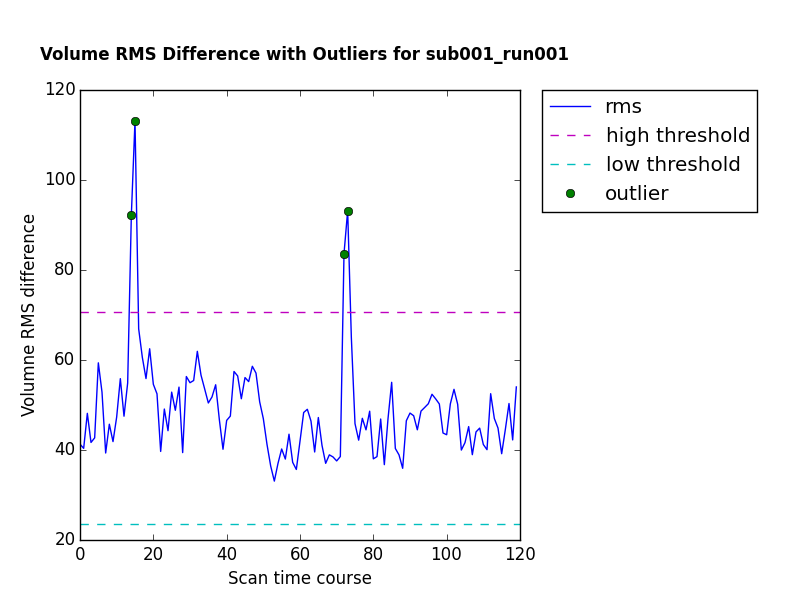
\includegraphics[width=90mm]{Volume_RMS_Difference_Outliers_sub001_run001.png}
\caption{Remove Outliers}
\end{figure}

Then, we generated task time course with the event2neural function.
\begin{figure}[h!]
\centering
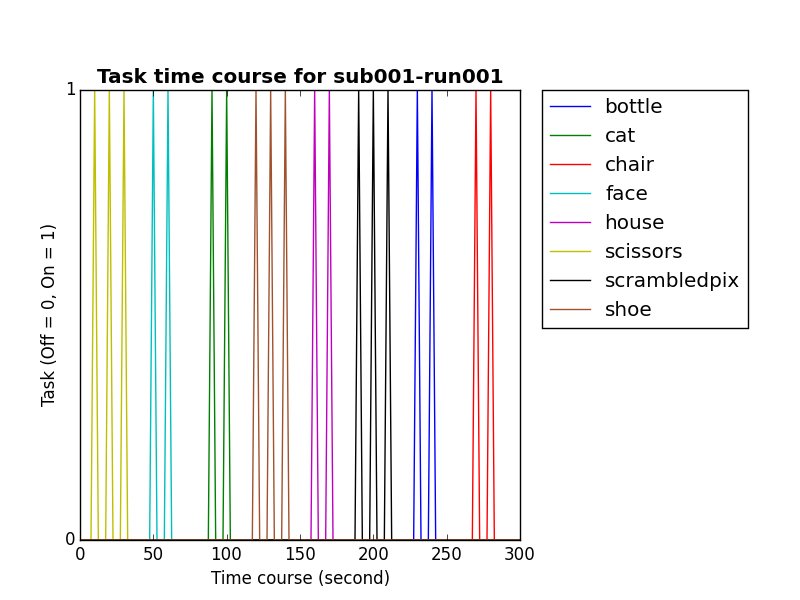
\includegraphics[width=90mm]{Task_time_course_sub001_run001.png}
\caption{Task Time Course}
\end{figure}

\pagebreak 

Afterwards, we performed convolution to generate predicted BOLD signals for this 
dataset.
\begin{figure}[h!]
\centering
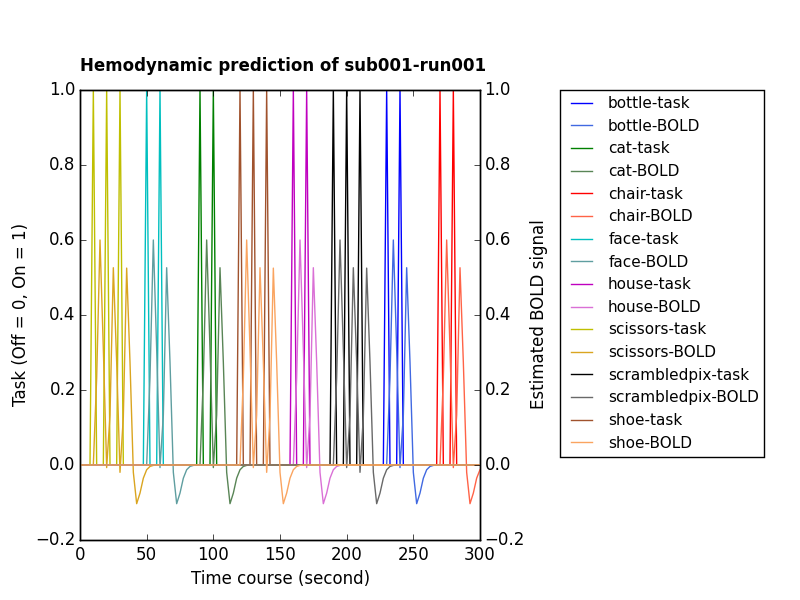
\includegraphics[width=100mm]{sub001_run001_bold_prediction.png}
\caption{Stimulation Bold}
\end{figure}

These convolved results for each objects were used as parameters in 
our design matrix for linear regression. To avoid the drifting problem, we also 
included two drift parameters in the design matrix. The final design matrix was 
arranged as followed: bottle, cat, chair, face, house, scissors, scrambledpix, 
shoe, drift1, drift2, average(all ones). 
\begin{figure}[h!]
\centering
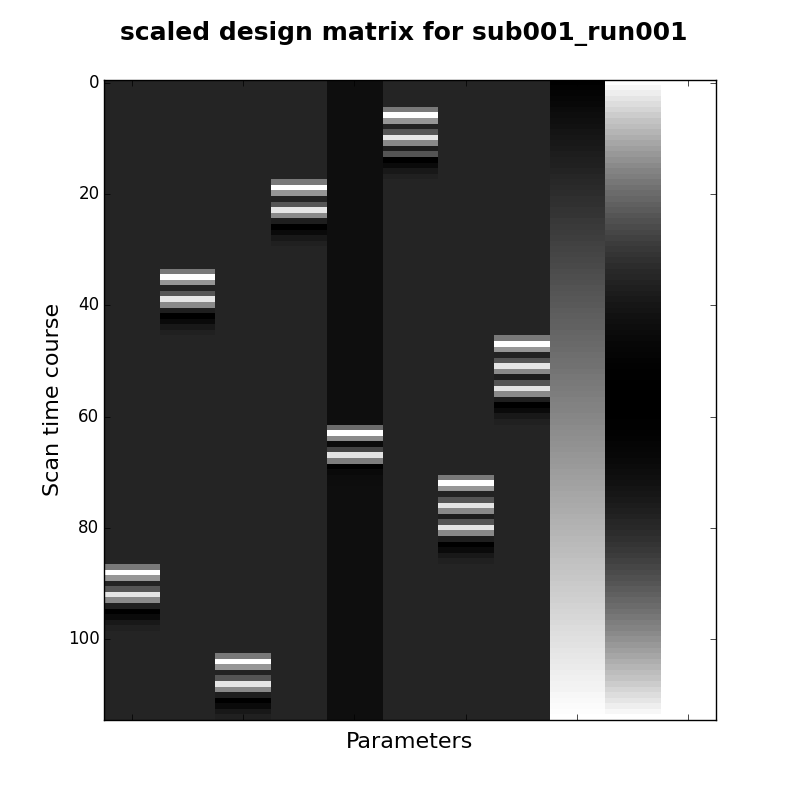
\includegraphics[width=90mm]{design_matrix_sub001_run001.png}
\caption{Design Matrix}
\end{figure}

As mentioned above, we ran correlation analysis on the beta values.
None of the correlation values are perfectly 1. The diagonal values 
are correlations between each object with their respective odd or 
even runs (within-category correlations). All within-category correlation 
values are larger than 0.6. For bottle, cat, face, house, scrambledpix, 
and shoe, the respective within-category correlations are higher than 
all of that object?s between-category correlations with other objects. 
For chair and scissors, the within-category correlations are not higher 
than all of their between-category correlations.
\begin{figure}[h!]
\centering
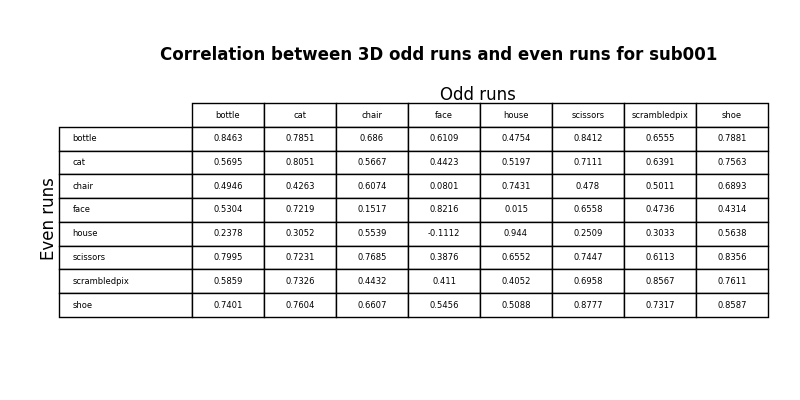
\includegraphics[width=90mm]{3d_correlation_table_sub001.png}
\caption{3D Correlation Table for Subject 1}
\end{figure}

\begin{figure}[h!]                                                              
\centering                                                                      
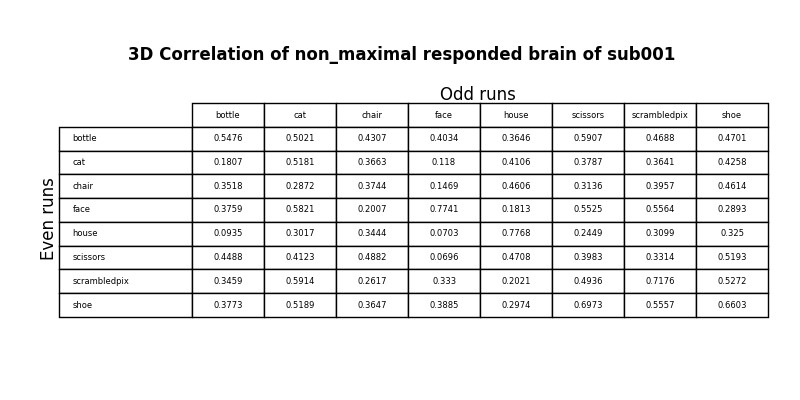
\includegraphics[width=90mm]{3d_non_max_correlation_table_sub001.png}                   
\caption{3D Correlation Excluding Maximally Responding Voxels for Subject 1}                                    
\end{figure}

\section{Discussion}

Most of the within-category correlations we found are fairly similar than the paper?s. 
Some of the values from our analysis are higher than the paper?s, which could be 
due to the fact that we only analyzed correlations between runs for one subject, 
while the original research paper studied all subjects. It would make sense that 
correlations are higher when only analyzing brain activity from one brain. \\

Correlations between different objects (between-category correlations) seem 
fairly random, which also seem to be in line with the original paper?s finding. 
We observe that our between-category correlation values also tend to be higher 
than those from the paper. \\

To test the reproducibility of the study, we also redid our correlation analysis 
after excluding the maximally-responsive voxels. With the exception of some 
within-category correlations, most correlation values across all categories dropped 
after we removed the maximally-responsive voxels. This might be an indication 
that most of the highly correlated areas tend to have higher responses. \\

There are a lot of problems that came up during our analysis. To begin with, 
since most of us have limited neuroscience knowledge, it was very difficult 
just to understand the study and the data itself. The research paper of the 
study uses specific and technical terms that make it hard to comprehend. 
More time was spent at the earlier stages of this project rereading the 
original paper and exploring the data folders than expected, which slowed down 
our progress for analysis. Therefore, we only had time to investigate one 
subject and one run so far. Now that we have a better understanding of the 
study and the data, we hope to repeat our analysis on the remaining subjects.\\

After we understood which part of the data to use, we started our 
exploratory data analysis. There is a lot of noise within the original dataset, 
causing insignificant p-values for test statistics, such as t-tests. Moreover, 
the noise in the original dataset produces low-resolution brain images, 
which are not meaningful for our further analysis. Pre-processing of data, 
including the removal of outliers using techniques from homework 2, was 
performed. In addition, we used smoothing techniques to create clearer 
and more meaningful images. \\

Furthermore, we faced problems recently that are yet to be resolved. Since 
subjects' heads often slowly move to a certain direction during fMRI scans, 
drifting of time series graph of BOLD signals is observed. We are planning 
to apply time series analysis modeling techniques, which will hopefully take 
the drifting into account and improve the accuracy of our models. Also, the 
BOLD signals change differs from subject to subject, making it difficult to 
compare signals from the same run between subjects. We would need to 
find a statistical valid way to standardize the BOLD signals, so we could 
analyze how BOLD signals under different conditions are related to each 
other across subjects. \\

\bibliography{project}

\section{Appendix}

\begin{figure}[h!]
\centering
\includegraphics[width=90mm, height = 90mm]%
{betas_for_sub001_run001_house.png}
\caption{Betas for Sub001 Run001}
\end{figure}

\begin{figure}[h!]
\centering
\includegraphics[width=90mm]%
{sub001_run_figure_compile.png}
\caption{Sub001 2D Compiled}
\end{figure}
\newpage

\begin{figure}[h!]
\centering
\includegraphics[width=90mm, height = 45mm]%
{sub001_2d_bottle_total_correlation_bar_both.png}
\caption{Sub001 2D Correlation: Bottle}
\end{figure}

\begin{figure}[h!]
\centering
\includegraphics[width=90mm, height = 43mm]%
{sub001_2d_cat_total_correlation_bar_both.png}
\caption{Sub001 2D Correlation: Cat}
\end{figure}

\begin{figure}[h!]
\centering
\includegraphics[width=90mm, height = 44mm]%
{sub001_2d_chair_total_correlation_bar_both.png}
\caption{Sub001 2D Correlation: Chair}
\end{figure}

\begin{figure}[h!]
\centering
\includegraphics[width=90mm, height = 43mm]%
{sub001_2d_face_total_correlation_bar_both.png}
\caption{Sub001 2D Correlation: Face}
\end{figure}

\begin{figure}[h!]
\centering
\includegraphics[width=90mm, height = 40mm]%
{sub001_2d_house_total_correlation_bar_both.png}
\caption{Sub001 2D Correlation: House}
\end{figure}

\begin{figure}[h!]
\centering
\includegraphics[width=90mm, height = 40mm]%
{sub001_2d_scissors_total_correlation_bar_both.png}
\caption{Sub001 2D Correlation: Scissor}
\end{figure}

\begin{figure}[h!]
\centering
\includegraphics[width=90mm, height = 40mm]%
{sub001_2d_scrambledpix_total_correlation_bar_both.png}
\caption{Sub001 2D Correlation: Scram}
\end{figure}

\begin{figure}[h!]
\centering
\includegraphics[width=90mm, height = 40mm]%
{sub001_2d_shoe_total_correlation_bar_both.png}
\caption{Sub001 2D Correlation: Shoe}
\end{figure}


\newpage


\begin{figure}[h!]
\centering
\includegraphics[width=90mm]%
{sub001_3d_bottle_total_correlation_bar_both.png}
\caption{Sub001 3D Correlation: Bottle}
\end{figure}

\begin{figure}[h!]
\centering
\includegraphics[width=90mm]%
{sub001_3d_cat_total_correlation_bar_both.png}
\caption{Sub001 3D Correlation: Cat}
\end{figure}

\begin{figure}[h!]
\centering
\includegraphics[width=90mm]%
{sub001_3d_chair_total_correlation_bar_both.png}
\caption{Sub001 3D Correlation: Chair}
\end{figure}

\begin{figure}[h!]
\centering
\includegraphics[width=90mm]%
{sub001_3d_face_total_correlation_bar_both.png}
\caption{Sub001 3D Correlation: Face}
\end{figure}

\begin{figure}[h!]
\centering
\includegraphics[width=90mm]%
{sub001_3d_house_total_correlation_bar_both.png}
\caption{Sub001 3D Correlation: House}
\end{figure}

\begin{figure}[h!]
\centering
\includegraphics[width=90mm]%
{sub001_3d_scissors_total_correlation_bar_both.png}
\caption{Sub001 3D Correlation: Scissor}
\end{figure}

\begin{figure}[h!]
\centering
\includegraphics[width=90mm]%
{sub001_3d_scrambledpix_total_correlation_bar_both.png}
\caption{Sub001 3D Correlation: Scram}
\end{figure}

\begin{figure}[h!]
\centering
\includegraphics[width=90mm]%
{sub001_3d_shoe_total_correlation_bar_both.png}
\caption{Sub001 3D Correlation: Shoe}
\end{figure}
\newpage

\begin{figure}[!h]
\centering
\includegraphics[width=90mm, height = 43mm]%
{2d_total_correlation_bar_both_bottle.png}
\caption{Cross Subject 2D Correlation: Bottle}
\end{figure}

\begin{figure}[h!]
\centering
\includegraphics[width=90mm, height = 44mm]%
{2d_total_correlation_bar_both_cat.png}
\caption{Cross Subject 2D Correlation: Cat}
\end{figure}

\begin{figure}[h!]
\centering
\includegraphics[width=90mm, height = 43mm]%
{2d_total_correlation_bar_both_chair.png}
\caption{Cross Subject 2D Correlation: Chair}
\end{figure}

\begin{figure}[h!]
\centering
\includegraphics[width=90mm, height = 44mm]%
{2d_total_correlation_bar_both_face.png}
\caption{Cross Subject 2D Correlation: Face}
\end{figure}

\begin{figure}[h!]
\centering
\includegraphics[width=90mm]%
{2d_total_correlation_bar_both_house.png}
\caption{Cross Subject 2D Correlation: House}
\end{figure}

\begin{figure}[h!]
\centering
\includegraphics[width=90mm]%
{2d_total_correlation_bar_both_scrambledpix.png}
\caption{Cross Subject 2D Correlation: Scram}
\end{figure}

\begin{figure}[h!]
\centering
\includegraphics[width=90mm]%
{2d_total_correlation_bar_both_shoe.png}
\caption{Cross Subject 2D Correlation: Shoe}
\end{figure}

\begin{figure}[h!]
\centering
\includegraphics[width=90mm]%
{2d_total_correlation_bar_both_scissors.png}
\caption{Cross Subject 2D Correlation: Scissors}
\end{figure}

\newpage

\begin{figure}[h!]
\centering
\includegraphics[width=90mm]%
{3d_total_correlation_bar_both_bottle.png}
\caption{Cross Subject 3D Correlation: Bottle}
\end{figure}

\begin{figure}[h!]
\centering
\includegraphics[width=90mm]%
{3d_total_correlation_bar_both_cat.png}
\caption{Cross Subject 3D Correlation: Cat}
\end{figure}

\begin{figure}[h!]
\centering
\includegraphics[width=90mm]%
{3d_total_correlation_bar_both_chair.png}
\caption{Cross Subject 3D Correlation: Cat}
\end{figure}

\begin{figure}[h!]
\centering
\includegraphics[width=90mm]%
{3d_total_correlation_bar_both_face.png}
\caption{Cross Subject 3D Correlation: face}
\end{figure}

\begin{figure}[h!]
\centering
\includegraphics[width=90mm]%
{3d_total_correlation_bar_both_house.png}
\caption{Cross Subject 3D Correlation: House}
\end{figure}

\begin{figure}[h!]
\centering
\includegraphics[width=90mm]%
{3d_total_correlation_bar_both_scrambledpix.png}
\caption{Cross Subject 3D Correlation: Scram}
\end{figure}

\begin{figure}[h!]
\centering
\includegraphics[width=90mm]%
{3d_total_correlation_bar_both_shoe.png}
\caption{Cross Subject 3D Correlation: shoe}
\end{figure}

\begin{figure}[h!]
\centering
\includegraphics[width=90mm]%
{3d_total_correlation_bar_both_scissors.png}
\caption{Cross Subject 3D Correlation: Scissors}
\end{figure}

\end{document}
